\chapter{Implementação}
\label{chap:imp}

\section{Introdução}
\label{chap4:sec:intro}

\section{Linguagens de Programação}
\label{chap3:linguagens}
Tal como o título deste projeto sugere, \textbf{\emph{Go}} (frequentemente referido como \emph{Golang}) é a linguagem usada na implementação do protocolo. Para além de \emph{Go}, também foi utilizada \textbf{\emph{JavaScript}} como linguagem de implementação da visualização.

De seguida serão descritas as razões de utilização da linguagem Go e brevemente detalhes sobre o uso de \emph{JavaScript}:



\subsection*{\emph{Go}}

A implementação de \textbf{sistemas concorrentes} em \emph{Go} é \textbf{simples}, sendo a razão príncipal para a utilização desta tecnologia. 
Adicionando a palavra ``\emph{go}'' antes de qualquer procedimento, esse procedimento irá correr em uma nova \emph{Goroutine}, de forma concorrente em relação a todas as outras \emph{Goroutines} já em execução.
Uma ``Goroutine'' é um \emph{lightweight \textbf{thread}} gerido pelo \emph{runtime} do \emph{Go}.


% Mudar, pouco informativo
%Outras razões são:
%\begin{description}
    %\item [Simplicidade] Desenhada para ter o mínimo de funcionalidades (apenas as necessárias) e ser fácil de ler
    %\item [Rapidez] o código é compilado em código de máquina.
%\end{description}


Por exemplo, comparando (parcialmente) \emph{Go} e \emph{Java}, um programa concorrente que mostra os números inteiros de 0 a 10:
\begin{lstlisting}[caption={Exemplo em \emph{Go}, usando a \emph{keyword} ``go'' para começar uma \emph{Goroutine}.},language=Go]
func main() {
	var wg sync.WaitGroup
	wg.Add(2)

	go count(&wg, "Goroutine-1")
	go count(&wg, "Goroutine-2")


	wg.Wait()
}

func count(wg *sync.WaitGroup, goroutineName string) {
	defer wg.Done()
	for i := 0; i < 10; i++ {
		fmt.Printf("Thread %s, %d\n", goroutineName, i)
		time.Sleep(time.Second * 40)
	}
}
\end{lstlisting}

% adicionar à biografia https://www.tutorialspoint.com/java/java_multithreading.htm

\begin{lstlisting}[caption={Exemplo em \emph{Java}, usando a \emph{interface} ``Runnable'' e uma classe``RunnableDemo'' para começar \emph{threads}.},language=Java]
class RunnableDemo implements Runnable {
   private Thread t;
   private String threadName;
   
   RunnableDemo( String name) {
      threadName = name;
   }
   public void run() {
      try {
         for(int i = 10; i < 10; i++) {
            System.out.println("Thread: " + threadName + ", " + i);
            Thread.sleep(40);
         }
      } catch (InterruptedException e) {
         System.out.println("Thread " +  threadName + " interrupted.");
      }
   }
   public void start () {
      if (t == null) {
         t = new Thread (this, threadName);
         t.start ();
      }
   }
}

public class TestThread {

   public static void main(String args[]) {
      RunnableDemo R1 = new RunnableDemo( "Thread-1");
      R1.start();
      
      RunnableDemo R2 = new RunnableDemo( "Thread-2");
      R2.start();
   }   
}

\end{lstlisting}

Além da simplicidade de especificação de procedimentos concorrentes, a linguagem oferece bibliotecas de apoio a programas concorrentes, como a biblioteca ``sync'' que disponibiliza primitivas de sincronização simples (como por exemplo \emph{WaitGroups} e \emph{Mutex Locks}), e canais que permitem a comunicação e partilha de dados entre \emph{Goroutines}.

A concorrência é inerente aos sistemas distribuídos, visto que os vários elementos do sistema executam de forma independente e em simultâneo.

Um exemplo relacionado com o tema deste projeto seria o caso em que um \emph{Node} recebe vários pedidos de outros \emph{Nodes}. De forma a manter o sistema (ou o diretório) consistente , o \emph{Node} que recebeu os pedidos terá de os tratar de forma sincronizada, isto é, tem de abordar um pedido de cada vez.

Na implementação fez-se uso de servidores e pedidos \acs{HTTP}. Por omissão, todos os pedidos \acs{HTTP} que o servidor recebe são tratados em \emph{goroutines} diferente, o que permite a receção dos vários pedidos e para a sincronização das \emph{goroutines} usou-se um ``Mutex'' proveniente da biblioteca ``sync''.

%Também é possível que vários elementos enviem pedidos ao mesmo tempo, e cada \emph{Node} age de forma independente e não tem informação sobre o resto do sistema (excepto os vizinhos), então executa em simultâneo com outros \emph{Nodes}.



\subsection*{\emph{JavaScript}}
Para a implementação da visualização foi usado \textbf{JavaScript}.
Esta linguagem permite que a informação de páginas \emph{Web} seja alterada após o seu carregamento.
É usado no desenho de grafos e alteração de tabelas que dispõem a informação da visualização da rede.



\section{Ferramentas e Bibliotecas utilizadas}
\subsection*{Ferramentas}
As ferramentas usadas durante a implentação deste projeto foram:
\begin{description}
    \item [GoLand] \acs{IDE} especializado para \emph{Go}. Inclui \emph{Plugins} de \emph{Debugging}, sugestão de código, etc.
    \item [VIM] Editor de texto/conjunto de atalhos de teclado. Permite escrever texto de forma eficiente e apenas usando o teclado. Pode ser usado como \emph{Plugin} no \acs{IDE} \emph{GoLand}.
    \item [GitHub] Esta plataforma foi útil no controlo de versões do projeto e na partilha do código e especificação do protocolo.
\end{description}

\subsection*{Bibliotecas}
\label{chap3:bibliotecas}
Nesta secção irão ser referidas bibliotecas utilizadas na implementação e as suas funcionalidades.

\subsubsection*{\emph{gorilla/mux}}
Multiplexador de pedidos \acs{HTTP}. Esta biblioteca da linguagem \emph{Go} foi utilizada para simplificar a declaração de caminhos do servidor \acs{HTTP}. É usada nos \emph{Nodes} e no servidor \acs{HTTP} da visualização.

\subsubsection*{\emph{D3.JS}}
A biblioteca \emph{D3.JS}, em que \emph{D3} significa ``\emph{\textbf{D}ata-\textbf{D}riven \textbf{D}ocuments}'', em português, ``documentos dirigidos em dados'', é usada para a representar gráficamente dados.
No contexto deste projeto, esta é utilizada para a visualização da rede que estamos a testar, sendo que esta é representada como um grafo.
Esta biblioteca permite a atualização periódica da representação do estado da rede de forma simples.
Faz uso do elemento \emph{\acs{SVG}} do \emph{\acs{HTML}}, que é um \emph{Standard}, o que permite a funcionalidade desta em grande maioria dos \emph{Browsers} modernos, e é ``leve'', a qual nos possibilita uma grande taxa de atualização do grafo com dados mais recentes.

\subsection*{Outras Tecnologias}
\label{chap3:outras_tecnologias}
\subsubsection*{\emph{Docker}}

Docker é uma plataforma aberta/ferramenta construída de forma a tornar mais acessível a criação e execução de programas  usando \emph{containers}.

% explicar melhor containers

Estes \emph{containers} podem ser comparados com \emph{Virtual Machines}, ambos tendo o mesmo propósito, mas os \emph{containers} \emph{Docker} são mais leves, mais rápidos e portáveis.


No entanto, esta tecnologia foi utilizada para simular uma rede distribuída, em que cada \emph{container} simula um \emph{Node} ou uma máquina que cada um tem uma instância do programa a correr, o seu próprio endereço \acs{IP} e que podem comunicar entre si.




%\section{Escolhas de Implementação}
%\label{chap4:escolhas_implementacao}
% Explicar o uso das bibliotecas
% Explicar a necessidade da visualização
% Explicar o uso de pedidos HTTP (por ser um contexto distribuido, e HTTP ser um dos protocolos mais usados
% Explicar uso de Containers Docker


\section{Classe \emph{Node}}
A Classe \emph{Node} desempenha a função de armazenar o estado atual do próprio \emph{Node}, define os métodos/procedimentos que este pode executar, e uma enumeração dos 5 diferentes tipos de \emph{Nodes}.



Nesta Implementação, esta classe está incluída num módulo \emph{Go} ``Nodes'' (Ou seja, num diretório com o mesmo nome), e é constituído por 5 ficheiros, sendo que o código está distribuído por entre os ficheiros da seguinte forma:

\begin{description}
    \item [Node.go] - Contém \emph{Struct} que define os \textbf{atributos}.
    \item [NodeBehaviours.go] - Define os possíveis \textbf{comportamentos}.
    \item [NodeCommunications.go] - Conjunto de \textbf{métodos de comunicação} de informação para outros \emph{Nodes}.
    \item [NodeTranformations.go] - \textbf{Transformações}/Mudanças de tipo que o \emph{Node} pode sofrer.
    \item [NodeType.go] - Enumeração dos \textbf{tipos} que o \emph{Node} pode ser.
\end{description} 


\section{Atributos da Classe}
Como referido no capítulo de Especificação, um \emph{Node} tem, no máximo 5 atributos, no entanto, na sua implementação este incluí no total 8, tendo a mais os atributos ``MyAddress'', ``Type'' e ``VisAddress''.
Esta é a definição da \emph{Struct} dos atributos do \emph{Node}.


Este código está presente no ficheiro Node.go.


\begin{lstlisting}[caption={Definição da estrutura \emph{Node}},language=Go]
type Node struct {
	Type       NodeType //Tipo do Node, ver Tipos de Nodes
	MyChan     string   //Channel onde recebe acesso ao objeto
	Find       string   //Channel onde recebe pedidos
	Link       string   //Ligacao para o child Node
	WaiterChan string   //Channel do Node que esta na posicao seguinte da fila
	MyAddress  string   //Endereco do Node
	VisAddress string   //Endereco para onde envia o seu estado atual para a atualizacao da visualizacao
	Obj        bool     //Se tem objeto ou nao 
}

\end{lstlisting}
Na \emph{Struct} estão definidos todos os atributos que o \emph{Node} pode ter, porém, quando um atributo é inexistente, este é definido como vazio, ou seja, os atributos ``WaiterChan'', ``VisAddress'' e ``Link'' podem ser \emph{strings} vazias.

O atributo \textbf{``MyChan''} é o \emph{Channel} do \emph{Node} onde este vai receber o acesso ao objeto.
Também é usado na construção da \emph{Struct} que irá ser enviada para o \emph{Child} node quando este decide pedir o acesso ao objeto.

O atributo \textbf{``Find''} é o \emph{Channel} do \emph{Node} onde este vai receber pedidos de acesso de outros \emph{Nodes}. 
Também é usado na construção dos dois tipos de pedidos, no pedido de \emph{AccessRequest} quando o \emph{Node} decide fazer um pedido e quando este reencaminha um pedido para o \emph{Child Node}, ao construir um novo pedido de \emph{AccessRequest}, mantendo o ``WaiterChan'' mas substituindo o ``Link'' do pedido pelo seu ``Find''.

O atributo \textbf{``Link''} é o \emph{Channel ``Find''} do \emph{Child Node}. Pode existir ou não, caso não exista este é representado como uma \emph{string} vazia.
Este é usado para o reencaminhamento e difusão de quaisquer pedidos ``AccessRequest'', quer estes sejam construídos pelo \emph{Node} ou pedidos que chegaram ao seu ``Find''.

O atributo \textbf{``WaiterChan''} é o \emph{Channel ``MyChan''} do \emph{Node} que espera pelo acesso ao objeto. Pode existir ou não, caso não exista este é representado como uma \emph{string} vazia.
Este é usado na atribuição do objeto ao \emph{Node} que está à espera do acesso ao objeto, por parte do \emph{Node}.

O atributo \textbf{``MyAddress''} é o endereço \acs{IP} do próprio Node. 
Este é usado para identificação do \emph{Node} na rede e para a construção dos \emph{Channels ``Find''} e \emph{``MyChan''},
pois este é usado na inicialização do servidor \acs{HTTP} do \emph{Node}.

O atributo \textbf{``VisAddress''} é o \acs{URL} usado para a atualização do estado do \emph{Node} na visualização.

O atributo \textbf{``Obj''} apenas indica se o \emph{Node} tem acesso ou não ao objeto.
Este atributo é redundante, pois a mesma informação pode ser adquirida a partir do tipo do node (``Type''), 
em que, caso o \emph{Node} seja do tipo \emph{OwnerTerminal} ou \emph{OwnerWithRequest}, este tem o acesso ao objeto.


\section{Inicialização do objeto ``Self Node''}

Nesta secção será descrito o processo de inicialização do objeto ``Self Node'', 
isto é, a definição dos atributos do \emph{Node} que o programa irá definir.

Para tal, os atributos do \emph{Node} provêm de argumentos da linha de comandos, isto para facilitar
a inicialização de \emph{Nodes} sem interface gráfica ou com uso de ``scripts''/``Dockerfiles'' (Ficheiros de construção de imagens \emph{Docker}).

Na linguagem ``Go'' existe uma função especial, ``init'', que é sempre executada (e a primeira) no carregamento de um módulo \emph{Go},
que foi usada para garantir que a inicialização do \emph{Node} esteja completa antes da execução de qualquer outra função.



Nesta função, é instanciado o objeto ``selfNode'' da classe ``Node'', e é armazenado o ponteiro para o mesmo, para que possa haver alteração do mesmo
por parte dos seus métodos.

Os argumentos da linha de comandos são analisados/\emph{Parsed} e transformados/\emph{Casted} de texto para o tipo
correspondente ao do atributo (por exemplo, o tipo é \emph{Casted} de texto para um inteiro), sendo que 
os únicos atributos não opcionais são o endereço (``MyAddress'') do \emph{Node} e o seu tipo.


\begin{lstlisting}[caption={\emph{Parsing} dos argumentos da linha de comandos.},language=Go]
	selfNode = new(Nodes.Node) //Instanciacao do ``selfNode'' e armazenamento do ponteiro para o mesmo

	// \emph{Parsing} dos argumentos da linha de comandos
	// as funcoes do modulo ``flag'' devolvem ponteiros para a instanciacao de cada argumento \emph{Parsed}
	myAddress := flag.String("address", "", "Node's Address (Required)")
	myType := flag.Int("type", -1, "Node's Type (0-4)(Required)") //Por definicao de todos os tipos
	visAddress := flag.String("visualization", "", "Visualization address.")
	link := flag.String("link", "", "Link")
	requests := flag.Bool("requests", true, "If this Node, when Idle, preforms Object Requests")

	// Chamado apos todas as ``flags'' serem definidas, para que seja processado o \emph{Parsing}
	flag.Parse()

\end{lstlisting}

No entanto, atributos como ``Link'', ``MyChan'', ``Find'', e ``Type'' que dependem do endereço dos \emph{Nodes},
que apenas são formados se o \emph{Parsing} for bem sucedido.

Dependendo do tipo do \emph{Node}, irão ser executas instruções para garantir o bom funcionamento do diretório/simulação,
como por exemplo, caso o \emph{Node} seja do tipo ``OWNER'', é definido que este tem o objeto implicitamente, ou
caso seja do tipo ``IDLE'' irá ser inicializada uma \emph{goroutine} que executará o método ``AutoRequest'' do \emph{Node},
para que este tenha a possibilidade de realizar pedidos automáticamente/aleatoriamente.

% Mudar os comentários
\begin{lstlisting}[caption={Instanciação dos atributos do \emph{Node}.},language=Go]

	selfNode.MyAddress = *myAddress

	// instanciacao dos \emph{Channels ``Find''} e \emph{``MyChan''}
	// concatenacao de ``http://'' que indica ao \emph{Node} que transmitira o pedido que este deve ser um pedido \acs{HTTP}
	// concatenacao dos caminhos ``/find'' e ``/myChan'' para indicar aos \emph{Nodes} para que \emph{Channel} sera enviado

	selfNode.MyChan = fmt.Sprintf("http://%s/myChan", *myAddress)
	selfNode.Find = fmt.Sprintf("http://%s/find", *myAddress)

	selfNode.Type = Nodes.NodeType(*myType)



	selfNode.VisAddress = fmt.Sprintf("http://%s", *visAddress)

	selfNode.Link = *link
	if *link != "" {
		selfNode.Link = fmt.Sprintf("http://%s/find", *link)
	}

	// Caso seja do tipo ``OWNER'', o \emph{Node} tem o acesso ao objeto
	if selfNode.Type == Nodes.OWNER_TERMINAL || selfNode.Type == Nodes.OWNER_WITH_REQUEST {
		selfNode.Obj = true


		//caso seja ``IDLE'', sera executado o metodo ``AutoRequest'' numa nova \emph{Goroutine}
	} else if selfNode.Type == Nodes.IDLE && *requests{ 
		go selfNode.AutoRequest()
	}

\end{lstlisting}


\section{Tipos de Nodes}
\label{chap:imp:node:tipos}
% Pouco informativo

Os 5 tipos de \emph{Nodes} foram definidos em uma enumeração de constantes inteiras.
\begin{lstlisting}[caption={Definição da enumeração dos tipos de \emph{Node}},language=Go]
type NodeType int


const (
	OWNER_WITH_REQUEST NodeType = iota //0
	OWNER_TERMINAL                     //1
	IDLE                               //2
	WAITER_WITH_REQUEST                //3
	WAITER_TERMINAL					   //4
)

\end{lstlisting}

\section{Comportamentos}
Como referido no capítulo de Especificação \ref{especificacao:atr:section}, 
o \emph{Node} pode ter vários comportamentos, 
que dependem do seu tipo e de fatores que os desencadeiam, como por exemplo receber um pedido de acesso ou o acesso ao objeto e 
o próprio \emph{Node} (no caso desta implementação) tomar decisões, como ceder o acesso ao objeto ou pedir o mesmo.

Este código está presente no ficheiro NodeBehaviours.go .

\subsection*{Receção de um pedido Access Request}
Todos os tipos de \emph{Nodes} têm a possibilidade de receber um pedido de \emph{AccessRequest}, no entanto, o comportamento (e transformação) desencadeado por este evento é diferente entre tipos.

% Referir a outra secção
Quando o \emph{Node} recebe um pedido \emph{Access Request} (\emph{Handler} ``findRoute'' no ficheiro ``controller.go'') o
e método ``HandleFind'' da classe \emph{Node} é executado.
O objeto de entrada provêm da descodificação dos dados transmitidos pelo \emph{Parent Node}.

Na implementação deste método, foi usada a estrutura condicional ``Switch'' para escolher que comportamento será tomado 
dependendo do tipo atual do ``selfNode''.

% Referir a outra secção
O acesso à secção crítica deste método é sincronizada com o uso do \emph{Mutex} ``Mutex'', isto é,
o acesso ao estado atual do ``selfNode'' só é adquirido por uma \emph{goroutine} de cada vez.

O pedido de \emph{Access Request} recebido, ``accessRequest'' é copiado para um novo objeto ``newAccessRequest'',
quer irá ser utilizado na construção de um novo ``AccessRequest'',
caso o \emph{Node} redirecione o pedido para o seu \emph{Child Node}.

% Referir a outra secção
O último procedimento a ser executado neste método é o método ``UpdateVisualization'' da classe ``Node'', em uma nova \emph{goroutine}.
Este método é usado para atualizar o estado atual do \emph{Node} na visualização.

\begin{lstlisting}[caption={\emph{Switch} de decisão do comportamento.},language=Go]
Mutex.Lock() // fecho do Mutex
defer Mutex.Unlock() // a primitiva defer indica que o codigo de abertura do Mutex sera corrido caso a execucao deste metodo termine

newAccessRequest := accessRequest // copia do pedido

// Decisao do comportamento que depende do tipo "Type" atual do Node
switch node.Type {
	case OWNER_TERMINAL:
	case OWNER_WITH_REQUEST:
	case IDLE:
	case WAITER_TERMINAL:
	case WAITER_WITH_REQUEST:
	}
go node.UpdateVisualization()
\end{lstlisting}

Será feita uma descrição do comportamento que cada tipo de \emph{Node} pode ter,
isto é, a implementação de cada caso do ``Switch''.

\subsubsection*{Caso OWNER\textunderscore TERMINAL}
% Referir a outra secção
Caso o tipo seja ``OWNER\textunderscore TERMINAL'', o \emph{Node}, o método ``OwnerWithRequest'' da classe \emph{Node} irá ser executado, que transforma o 
\emph{Node} em \emph{Owner With Request}.

Os parâmetros de entrada desse método serão o ``Link'' e ``WaiterChan'' (do atributo ``GiveAccess'' do pedido), que correspondem ao ``Find'' do \emph{Parent Node} e ao ``MyChan'' do \emph{Node} que fez o pedido, respetivamente.
Isto é, a ligação entre o \emph{Node} e o transmissor do pedido inverte-se, e o \emph{Node} passa a ter um \emph{Node} em espera.

% Referir a outra secção
Após a transformação, será executado o método ``releaseObj'' do \emph{Node}, que irá despoletar o comportamento de Cedência do Objeto, em uma nova \emph{goroutine}.


\begin{lstlisting}[caption={Comportamento do \emph{Node} tipo \emph{Owner Terminal} caso receba um pedido \emph{Access Request} no \emph{Channel ``Find''}},language=Go]
node.OwnerWithRequest(accessRequest.Link, accessRequest.GiveAccess.WaiterChan) // transfomacao em Owner With Request
go node.releaseObj() //comportamento de Cedencia do Objeto
\end{lstlisting}



\subsubsection*{Caso OWNER\textunderscore WITH\textunderscore REQUEST}
Caso o tipo seja ``OWNER\textunderscore WITH\textunderscore REQUEST'',
o Atributo ``Link'' do objeto ``newAccessRequest'' será substituído pelo ``Find'' do \emph{Node}, para o seu \emph{Child Node} inverter a ligação.

Após feita esta alteração do objeto, o \emph{Node} envia o objeto ``newAccessRequest'' pelo seu ``Link'' para o seu \emph{Child Node}.

Por último, o método ``OwnerWithRequest'' da classe \emph{Node} irá ser executado, em que o \emph{Node} mantém o tipo mas
é feita uma alteração do seu ``Link'' para o ``Find'' que provêm do pedido ``Access Request'' que recebeu, isto é, para o ``Find'' do seu \emph{Parent Node}, 
invertendo a ligação,
mas mantendo o \emph{WaiterChan} porque o \emph{Node} que fez o pedido ainda não tem o acesso ao objeto.


\begin{lstlisting}[caption={Comportamento do \emph{Node} tipo \emph{Owner With Request} caso receba um pedido \emph{Access Request} no \emph{Channel ``Find''}},language=Go]
//alteracao do ``Link'' do novo pedido para o ``Find'' do \emph{Node}
newAccessRequest.Link = node.Find 
// Transmissao do ``newAccessRequest'' pelo ``Link''
node.SendThroughLink(newAccessRequest) 
// Transformacao \emph{OwnerWithRequest}, que mantem o ``WaiterChan'', mas atualiza o ``Link''
node.OwnerWithRequest(accessRequest.Link, node.WaiterChan)
\end{lstlisting}



\subsubsection*{Caso IDLE}
Caso o tipo seja ``IDLE'',
o Atributo ``Link'' do objeto ``newAccessRequest'' será substituído pelo ``Find'' do \emph{Node}, para o seu \emph{Child Node} inverter a ligação.

Após feita esta alteração do objeto, o \emph{Node} envia o objeto ``newAccessRequest'' pelo seu ``Link'' para o seu \emph{Child Node}.

Por último,  método ``Idle'' da classe \emph{Node} irá ser executado, que mantém o tipo do \emph{Node}, mas
é feita a alteração do seu ``Link'' para o ``Find'' que provêm do pedido ``Access Request'' que recebeu, ou seja, para o ``Find'' do seu \emph{Parent Node}, 
que inverte a ligação.


\begin{lstlisting}[caption={Comportamento do \emph{Node} tipo \emph{Idle} caso receba um pedido \emph{Access Request} no \emph{Channel ``Find''}},language=Go]
//alteracao do ``Link'' do novo pedido para o ``Find'' do \emph{Node}
newAccessRequest.Link = node.Find
// Transmissao do ``newAccessRequest'' pelo ``Link''
node.SendThroughLink(newAccessRequest)
// Transformacao \emph{Idle}, que atualiza o ``Link''
node.Idle(accessRequest.Link)

\end{lstlisting}


\subsubsection*{Caso WAITER\textunderscore TERMINAL}
Caso o tipo seja ``WAITER\textunderscore TERMINAL'', o \emph{Node} o método ``WaiterWithRequest'' do \emph{Node} será executado,
que transforma o \emph{Node} em \emph{WAITER\textunderscore WITH \textunderscore REQUEST}.

Os parâmetros de entrada são o ``Link'' e ``WaiterChan'' (do atributo ``GiveAccess'' do pedido), que correspondem ao ``Find'' do \emph{Parent Node} e ao ``MyChan'' do \emph{Node} que fez o pedido, respetivamente.
O ``Link'' é o ``Find'' do \emph{Parent Node}, o que causa a inversão da ligação.

\begin{lstlisting}[caption={Comportamento do \emph{Node} tipo \emph{Waiter Terminal} caso receba um pedido \emph{Access Request} no \emph{Channel ``Find''}},language=Go]

// Transformacao \emph{OwnerWithRequest}, que mantem o ``WaiterChan'', mas atualiza o ``Link''.
node.WaiterWithRequest(accessRequest.Link, accessRequest.GiveAccess.WaiterChan)
\end{lstlisting}


\subsubsection*{Caso WAITER\textunderscore WITH \textunderscore REQUEST}	
Caso o tipo seja ``WAITER\textunderscore WITH \textunderscore REQUEST'', o Atributo ``Link'' do objeto ``newAccessRequest'' será substituído pelo ``Find'' do \emph{Node},
para que o \emph{Child Node} possa inverter a sua ligação.

Após feita esta alteração do objeto, o \emph{Node} envia o objeto ``newAccessRequest'' pelo seu ``Link'' para o seu \emph{Child Node}.

Por último, este sofre uma transformação. O método ``WaiterWithRequest'' da classe \emph{Node} irá ser executado, 
em que é feita uma alteração do seu ``Link'' para o ``Find'' que provêm do pedido ``Access Request'' que recebeu, ou seja, para o ``Find'' do seu \emph{Parent Node}, 
mas mantêm o \emph{WaiterChan} porque o \emph{Node} que fez o pedido ainda não tem o acesso ao objeto.
O ``Link'' é o ``Find'' do \emph{Parent Node}, o que causa a inversão da ligação.

\begin{lstlisting}[caption={Comportamento do \emph{Node} tipo \emph{Waiter With Request} caso receba um pedido \emph{Access Request} no \emph{Channel ``Find''}},language=Go]
newAccessRequest.Link = node.Find // Alteracao do atributo Find do objeto newAccessRequest para o Find do Node
node.SendThroughLink(newAccessRequest) // Envio do objeto newAccessRequest pelo link
node.WaiterWithRequest(accessRequest.Link, node.WaiterChan) //transformacao do Node. Mantem-se o WaiterChan mas altera-se o Link
\end{lstlisting}

\subsection*{Cedência do Objeto}
No caso do \emph{Node} ser do tipo ``WAITER\textunderscore TERMINAL'' e receber um pedido ``Access Request'', 
este sofre uma transformação, muda de tipo para ``WAITER\textunderscore WITH\textunderscore REQUEST'' e passou a deter o atributo ``WaiterChan'' (``MyChan'' do \emph{Node} que fez o pedido).

% forma como esta frase está construída pode não estar bem
Esta secção de código é executada concorrentemente (numa \emph{goroutine}) com qualquer outras \emph{goroutines} 
que estejam a ser executadas,
isto para permitir que o \emph{Node} receba outros pedidos,
que os transmita, e que outros comportamentos ou transformações possam ocorrer 
enquanto este espera para ceder o acesso, isto é, enquanto que o \emph{Node} é ``OWNER\textunderscore WITH\textunderscore REQUEST''.


Referente a um caso real, o \emph{Node} transmitiria o objeto pelo \emph{Channel ``WaiterChan''}, quando, por exemplo, 
o acesso a este não fosse mais necessário.
No entanto, por questões de se pretender criar uma simulação deste protocolo, o \emph{Node} decide ceder o acesso ao objeto após um tempo aleatório (entre 1 a 2 segundos)
depois de receber o pedido para o seu acesso.

É executada a primitiva ``defer'' com o método ``Unlock'' do objeto ``Mutex'' para,
quando esta função terminar, o \emph{Mutex} ser desbloqueado, para que outras \emph{goroutines}
possam aceder ao estado atual do objeto.

\begin{lstlisting}[caption={\emph{Node} espera 1 ou 2 segundos antes de ceder o objeto.},language=Go]
	defer Mutex.Unlock() // o ``Mutex'' e desbloqueado quando a execucao deste metodo terminar
	randomSleep := utils.RandomRange(1, 2) // Gera um numero aleatorio, neste caso, 1 ou 2
	time.Sleep(time.Second * time.Duration(randomSleep)) // A \emph{goroutine} espera durante o tempo aleatorio gerado (em segundos)
\end{lstlisting}

De seguida é criado um objeto da classe/tipo ``GiveAccess'' que será transmitido para o \emph{Node} em espera 
através do ``WaiterChan''.

\begin{lstlisting}[caption={Criação do objeto ``accessObject'', da classe ``GiveAccess''},language=Go]
	accessObject := Channels.GiveAccess{WaiterChan: node.WaiterChan}
\end{lstlisting}


Este método (``releaseObj''), contém uma secção crítica,
pois acede ao objeto ``selfNode''. 
O acesso à secção crítica deste método é sincronizada com o uso do \emph{Mutex} ``Mutex'', ou seja,
o acesso ao estado atual do ``selfNode'' só é adquirido por uma \emph{goroutine} de cada vez, para prevenir a alteração do estado
enquanto que o \emph{Node} transmite o acesso ao objeto, 
e para que a transformação (método ``Idle'') ocorra de seguida ao \emph{Node} deixar de ter o acesso ao objeto.

%Referir sendObjectAccess
Quando tiver a possibilidade de aceder à secção crítica, este irá transmitir o acesso do objeto ao \emph{Node} em espera.
De seguida, como já não possui o acesso ao objeto, este sofre um transformação, mudando-se para um \emph{Node}
do tipo ``IDLE'', mantendo o ``Link''.

Como o \emph{Node} transformou-se em ``IDLE'', é inicializada uma \emph{goroutine} que executará o método ``AutoRequest''.
Este método desempenha a função de decidir se o \emph{Node} faz um pedido de acesso. 
%Referir mais à frente o autoRequest
No entanto, este é descrito num capítulo diferente.

De seguida, o procedimento a ser executado neste método é o método ``UpdateVisualization'' da classe ``Node'',
em uma nova \emph{goroutine}.
Este método é usado para atualizar o estado atual do \emph{Node} na visualização.


\begin{lstlisting}[caption={Acesso à secção crítica, transmição do Objeto, transformação em \emph{Node} ``IDLE'', \emph{goroutine} de decisão de pedido, e atualização na visualização},language=Go]
	Mutex.Lock() //Pedido de acesso a seccao critica
	node.SendObjectAccess(accessObject) //Transmissao do objeto, atraves do envio do objeto ``accessObject''
	node.Idle(node.Link) //transformacao em ``IDLE'', mas mantendo o ``Link''
	go node.AutoRequest() // goroutine que decidira se o \emph{Node} faz um pedido de acesso
	go node.UpdateVisualization() // atualiza o estado do Node na visualizacao

\end{lstlisting}


\subsection*{Realização de um pedido de acesso}
No caso do \emph{Node} ser do tipo ``IDLE'', este tem a possibilidade de pedir o acesso ao objeto.
Qualquer outro tipo de \emph{Node} não pode fazer pedidos de acesso.

Neste método há acesso ao estado atual do \emph{Node},
logo faz-se uso de um ``Mutex'' para o acesso ser sincronizado.

Como, a partir da visualização e da ``Shell'' do \emph{Node} é possível forçar o \emph{Node} 
a realizar um pedido, quando a \emph{goroutine} acede à secção crítica do método (acesso ao estado atual do \emph{Node})
é verificado se o tipo do \emph{Node} é ``IDLE''.


% Linguagem de Web pode estar incorreta
Caso seja do tipo ``IDLE'', irá ser instanciado um objeto do tipo ``Channels.AccessRequest'', em que o atributo
``Link'' contém o \emph{Channel ``Find''}  do próprio \emph{Node}, ou seja, o \acs{URL} do método
onde o \emph{Node} recebe os pedidos ``AccessRequest'', e
o atributo "GiveAccess" (do tipo ``Channels.GiveAccess''), que contém o \emph{Channel ``MyChan''} do próprio
\emph{Node}, o \acs{URL} do método
onde o \emph{Node} recebe o acesso ao objeto.
Depois da instanciação, é executado o método ``SendThroughLink'' do \emph{Node}, que envia o objeto 
pelo ``Link'' do \emph{Node} para o seu \emph{Child Node}.

O ``Link'' deste objeto servirá para o \emph{Child Node} do \emph{Node} inverter a ligação, isto é, 
para que o \emph{Child Node} possa fazer a ligação de volta para o \emph{Node}.

O atributo ``GiveAccess'' será usado pelo próximo \emph{Node} \emph{Terminal} (quer este seja \emph{Owner} ou \emph{Waiter}), 
para quando esse próximo \emph{Node} obtiver acesso ao objeto, este redirecioná-lo para o \emph{Node} que realizou o pedido.

Como o \emph{Node} realizou um pedido de acesso e espera pelo acesso ao objeto, este transforma-se em 
``WAITER\textunderscore TERMINAl'', deixando de ter ``Link''.

Por último, o \emph{Node} atualiza o seu estado na visualização em uma nova \emph{goroutine}.


\begin{lstlisting}[caption={Método ``Request''},language=Go]
func (node *Node) Request() {
	Mutex.Lock() // Sincronizacao do acesso a seccao critica
	defer Mutex.Unlock() // O metodo ``Unlock'' do objeto ``Mutex'' sera executado caso o metodo ``Request'' termine

	//Existe para evitar:
	//que ou o utilizador faca um request e o node ja mudou de tipo
	//que se faca um request a partir do metodo do Node de pedidos remotos
	if node.Type != IDLE {
		fmt.Printf("Can't request an object if not Idle.")
		return
	}
	fmt.Printf("Requesting.")

	//Instanciacao do pedido de acesso
	accessRequest := Channels.AccessRequest{
		GiveAccess: Channels.GiveAccess{
			WaiterChan: node.MyChan,
		},
		Link: node.Find,
	}

	//Envio do pedido de acesso
	node.SendThroughLink(accessRequest)


	//transfomacao em WaiterTerminal, visto que este espera pelo acesso
	node.WaiterTerminal()

	//atualizacao do estado atual do Node na visualizacao
	go node.UpdateVisualization()
}
\end{lstlisting}


É possível o utilizador provocar a realização do pedido pelo \emph{Node}. Pode ser feito a partir de uma 
``Shell'' que é iniciada com o programa,
ou através da visualização, ao clicar duas vezes no \emph{Node} do grafo correspondente ao \emph{Node} em questão.

No entanto, por questões de simulação do diretório, caso o estado inicial do \emph{Node}
ou este mude de tipo para ``IDLE'', 
é iniciada uma \emph{goroutine} que executa o método ``AutoRequest'' da classe \emph{Node}.

Neste método existe um ciclo ``infinito'', cuja a única condição de saída é o \emph{Node} realizar o pedido.

A cada ciclo é gerado um valor aleatório, que será, em segundos, o tempo que esta \emph{goroutine} irá esperar.

Após a espera, um outro valor aleatório é gerado (0 ou 1),
que indicará se o \emph{Node} irá fazer um pedido (ou seja, se será executado o método ``Request'' da classe ``Node'').


Caso faça o pedido (seja o valor 1), o ciclo irá terminar.
Caso contrário, o \emph{Node} terá de esperar um tempo aleatório até ao próximo ciclo.

\begin{lstlisting}[caption={Método ``AutoRequest''},language=Go]
func (node *Node) AutoRequest() {
	var randomSleep int

	// Ciclo infinito
	for {

		randomSleep = utils.RandomRange(5, 15) // E gerado um numero inteiro aleatorio entre 5 e 15

		fmt.Printf("\nTrying to Request the Object in %d seconds.", randomSleep)


		// A \emph{goroutine} espera durante o valor de ``randomSleep'' (em segundos)
		time.Sleep(time.Second * time.Duration(randomSleep))

		//E gerado um numero inteiro, 0 ou 1.
		//Caso o valor seja 1, o \emph{Node} ira realizar um pedido de acesso e o ciclo termina
		if requests := utils.RandomRange(0, 1); requests > 0 {
			node.Request()
			break
		} else {
			//Caso seja 0, o \emph{Node} ira gerar um numero inteiro aleatorio entre 5 e 20
			cooldown := utils.RandomRange(5, 20)
			fmt.Printf("Didn't request. Retrying in %d seconds.", cooldown)
			// A \emph{goroutine} espera durante o valor de ``cooldown'' (em segundos)
			time.Sleep(time.Second * time.Duration(cooldown))
		}
	}

}
\end{lstlisting}
Este método permite que \emph{Node} realize pedidos em tempo aleatório com uma chance de 50\%,
ou seja, há a possibilidade de o \emph{Node} não realizar um pedido.


\subsection*{Receção acesso ao objeto}
Caso o \emph{Node} seja do tipo \emph{WAITER\textunderscore TERMINAL} ou \emph{WAITER\textunderscore WITH\textunderscore REQUEST}
este pode receber o acesso ao objeto.

Quando o \emph{Node} recebe um pedido \emph{GiveAccess} (\emph{Handler} ``myChanRoute'' no ficheiro ``controller.go'') o
método ``ReceiveObj'' da classe \emph{Node} é executado.
O objeto de entrada do método provêm da descodificação dos dados transmitidos pelo \emph{Owner}
que cedeu o acesso ao objeto, isto é, uma desserialização dos dados provenientes de um método \acs{HTTP} ``POST''
num objeto do tipo ``GiveAccess''.


Como neste método, é feito um acesso ao estado atual do \emph{Node} e há transformações, 
o acesso a esta secção crítica é sincronizada com o uso de um \emph{Mutex}.
Para tal, é executado o método ``Lock'' do objeto ``Mutex''.
No fim da execução deste método é necessário desbloquear o ``Mutex'', para tal 
a primitiva ``defer'' é usada, que executará o método ``Unlock'' do objeto ``Mutex''.

Como este programa se trata de uma simulação, este objeto não tem qualquer uso,
no entanto, num caso de uso,
este objeto seria um \emph{Channel} de comunicação com um ficheiro/base de dados, ou qualquer outro
objeto em que o seu acesso seria sincronizado.


Quando o \emph{Node} é ``WAITER\_TERMINAL'', ao receber o acesso ao objeto,
este transforma-se em ``OWNER\_TERMINAL'', pois não tem nenhum outro \emph{Node} em espera.


Quando o \emph{Node} é ``WAITER\_WITH\_Request'', ao receber o acesso ao objeto,
este transforma-se em ``OWNER\_WITH\_REQUES'', pois ainda tem outro \emph{Node} em espera.
%Referir capitulo do release.
Com o \emph{Node} tem outro \emph{Node} à espera do acesso, é inicializada uma \emph{goroutine}
que irá executar o método ``releaseObj'' da classe \emph{Node}.


Ao final, é inicializada uma \emph{goroutine} que executará 
o método ``UpdateVisualization'', para que o estado do \emph{Node}
seja atualizado na visualização.


\begin{lstlisting}[caption={Método ``ReceiveObj''},language=Go]

func (node *Node) ReceiveObj(giveAccess Channels.GiveAccess) {
	Mutex.Lock() // Sincronizacao do acesso a seccao critica
	defer Mutex.Unlock() // O metodo ``Unlock'' do objeto ``Mutex'' sera executado caso o metodo ``Request'' termine

	fmt.Printf("Received Access:")
	fmt.Println(giveAccess)
	switch node.Type {
	case WAITER_TERMINAL:
		node.OwnerTerminal()
		break
	case WAITER_WITH_REQUEST:
		node.OwnerWithRequest(node.Link, node.WaiterChan)
		go node.releaseObj()
		break
	}

	go node.UpdateVisualization()

}

\end{lstlisting}

\section{Transformações do \emph{Node}}

% possivelmente adicionar diagrama para ficar mais completo
% por exemplo, IDLE -> recebeu pedido -> IDLE (mas muda o LINK)
% ou, OWNER -> cedeu o objeto -> IDLE(deixou de ter WaiterChan)


Neste capítulo serão descritas as transformações que o \emph{Node}
pode sofrer, tais como as suas implementações.


% mudar o executa qualquer comportamento
O \emph{Node} sofre transformações quando este executa qualquer comportamento, 
no entanto, uma transformação não significa uma mudança de tipo,
mas uma mudança de estado.

Estas são as possíveis transformações que o \emph{Node} pode sofrer:

\begin{figure}[!htb]
\centering
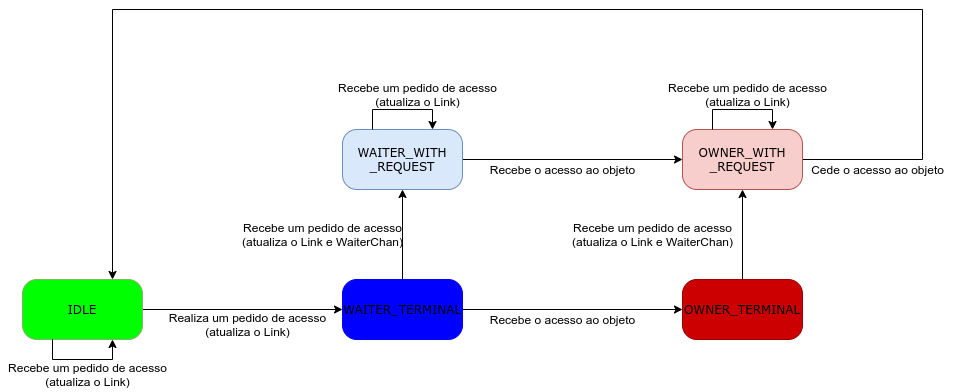
\includegraphics[width=500pt]{state-diagram.png}
\caption{Diagrama de Estados do \emph{Node}}
Nota: O estado inicial do \emph{Node} não está presente porque este pode começar em qualquer estado/tipo.
\end{figure}


O nome dos métodos das transformações provêm do nome to tipo 
para o qual se vai mudar ou manter.


\subsubsection*{Idle}
Se o \emph{Node} é do tipo ``IDLE'' e este recebe um pedido de acesso, após transmitir
o pedido para o seu \emph{Child Node}, sofre a transformação ``Idle'' (mantém o tipo) mas atualiza o \emph{Link} para o \emph{Find} do seu \emph{Parent Node}.
O novo ``Link'' (``NewLink'') é o parâmetro de entrada deste método.

Se o \emph{Node} é do tipo ``OWNER\_WITH\_REQUEST'' mas cedeu o acesso ao objeto, visto que este já não o possui o \emph{Node}
transforma-se em ``IDLE'', mas mantém o \emph{LINK}, isto é, o seu ``Link'' atual é usado como
parâmetro de entrada deste método.

\begin{lstlisting}[caption={Método/transformação ``Idle''},language=Go]
func (node *Node) Idle(newLink string) {
	node.Type = IDLE    //Alteracao do tipo para ``IDLE''
	node.Link = newLink //Atualizacao do ``Link''
	node.Obj = false    //Caso seja ``OWNER\_WITH\_REQUEST'', deixa de ter acesso ao obj
	node.WaiterChan = ""//Caso seja ``OWNER\_WITH\_REQUEST'', deixa de ter o ``Node'' em espera
}
	
\end{lstlisting}


\subsubsection*{WaiterTerminal}

Se o \emph{Node} é do tipo ``IDLE'' e realizar um pedido de acesso,
este sofre a transformação ``WaiterTerminal''.
Como foi o \emph{Node} que realizou o pedido de acesso, este não aponta para nenhum outro \emph{Node} (o ``Link'' passa a vazio/nulo).


\begin{lstlisting}[caption={Método/transformação ``WaiterTerminal''},language=Go]
func (node *Node) WaiterTerminal() {
	node.Type = WAITER_TERMINAL //Alteracao do tipo para ``WAITER\_TERMINAL''
	node.Link = ""       		// Como foi o \emph{Node} quem realizou o pedido, este nao aponta para nenhum outro \emph{Node}
	node.WaiterChan = "" 		//redundante
}
\end{lstlisting}



\subsubsection*{OwnerTerminal}

Se o \emph{Node} é do tipo ``WAITER\_TERMINAL'' e receber o acesso ao objeto, como
não recebeu qualquer pedido, este mantém-se sem ``Link'' ou ``WaiterChan'', 
então sofre a esta transformação, mudando o tipo para ``OWNER\_TERMINAL'', pois tem acesso ao objeto mas não tem qualquer pedido.

\begin{lstlisting}[caption={Método/transformação ``OwnerTerminal''},language=Go]
func (node *Node) OwnerTerminal() {
	node.Type = OWNER_TERMINAL //Alteracao do tipo para ``OWNER\{_}TERMINAL''
	node.Link = ""             
	node.Obj = true			   //Como se transformou em ``OWNER\{_}TERMINAL'' significa que passou a deter o acesso ao objeto
	node.WaiterChan = ""       //Redundante, mas um \emph{Node} deste tipo nao tem \emph{Node} a espera do acesso ao objeto
}
\end{lstlisting}

\subsubsection*{OwnerWithRequest}

Se o \emph{Node} é do tipo ``OWNER\_TERMINAL'' e receber um pedido de acesso, 
como este recebeu um pedido de acesso, o ``Link'' é atualizado e
como este é detentor do acesso ao objeto, o \emph{Node} passa a ter um pedido em espera, logo o ``WaiterChan'' é atualizado para o ``MyChan'' do \emph{Node} em espera.
Então sofre a transformação ``OwnerWithRequest'', mudando o tipo para ``OWNER\_WITH\_REQUEST'', sendo o ``NewLink'' e o ``WaiterChan'' os valores de entrada do método.

Caso o \emph{Node} seja do tipo ``OWNER\_WITH\_REQUEST'', ao receber um pedido de acesso, 
o ``Link'' é atualizado, pois, mesmo sendo o \emph{Node} com acesso ao objeto, este objeto será cedido a outro \emph{Node} e não ao
\emph{Node} que realizou o pedido.

\begin{lstlisting}[caption={Método/transformação ``OwnerWithRequest''},language=Go]
	func (node *Node) OwnerWithRequest(newLink string, waiterChan string) {
		node.Type = OWNER_WITH_REQUEST
		node.Link = newLink
		node.Obj = true
		node.WaiterChan = waiterChan
	}


\end{lstlisting}

\subsubsection*{WaiterWithRequest}

Se o \emph{Node} é do tipo ``WAITER\_TERMINAL'' e receber um pedido de acesso, 
como este recebeu um pedido de acesso, o ``Link'' é atualizado e
como este será detentor do acesso ao objeto, o \emph{Node} passa a ter um pedido em espera, logo o ``WaiterChan'' é atualizado para o ``MyChan'' do \emph{Node} em espera.
Então sofre a transformação ``WaiterWithRequest'', mudando o tipo para ``WAITER\_WITH\_REQUEST'', sendo o ``NewLink'' e o ``WaiterChan'' os valores de entrada do método.

Caso o \emph{Node} seja do tipo ``WAITER\_WITH\_REQUEST'', ao receber um pedido de acesso, 
o ``Link'' é atualizado, pois, mesmo que este \emph{Node} terá o acesso ao objeto, este objeto será cedido a outro \emph{Node} (do primeiro pedido que transformou o \emph{Node} em` `WAITER\_WITH\_REQUEST'' ) 
e não ao
\emph{Node} que realizou este pedido.

\begin{lstlisting}[caption={Método/transformação ``WaiterWithRequest''},language=Go]
	func (node *Node) WaiterWithRequest(newLink string, waiterChan string) {
		node.Type = WAITER_WITH_REQUEST
		node.Link = newLink
		node.WaiterChan = waiterChan
	}
	
\end{lstlisting}

\section{Comunicação entre Nodes}
% Explicar o uso de HTTP - industry standard

Neste capítulo serão tratadas as conexões que os \emph{Nodes} fazem entre si,
Como referido anteriormente, é feito uso do protocolo \acs{HTTP} nas ligação/pedidos entre \emph{Nodes}, pois este é um ``industry standard'' (ou seja, o protocolo mais usado neste tipo de sistemas).
Para tal, cada \emph{Node} inicia um servidor \acs{HTTP} que espera pela entrada de pedidos de HTTP, isto é, espera que outros \emph{Nodes} transmitam pedidos do tipo ``AccessRequest'' e ``GiveAccess''.
A implementação do servidor \acs{HTTP} está presente no módulo ``controller'' (no ficheiro ``controller.go'').

No entanto, também foram implementados métodos para permitir ao \emph{Node} a realização de pedidos, ou seja, de poder enviar informação para outros \emph{Nodes}.
A implementação destes pedidos \acs{HTTP} está presente no módulo ``Node'' (no ficheiro ``NodeCommunications.go'').


% acrescentar aqui mais alguma coisa

\subsection*{Servidor \acs{HTTP}}
Após a inicialização do programa do \emph{Node}, é inicializado o servidor \acs{HTTP}, executando a função ``StartServer'', em que é criado um objeto do tipo ``Router'' (roteador),  
no qual são registados os vários caminhos e \emph{Handlers}(manipuladores) destes caminhos. Isto é, são registados os métodos deste servidor e as funções que serão executadas
caso sejam feitos pedidos em cada um desses métodos.

Os métodos e \emph{Handlers} registados são:


\begin{description}
	\item [/find] findRoute \\ Saida do \emph{Channel ``Find''} do \emph{Node}
	\item [/myChan] myChanRoute \\ Saida do \emph{Channel ``MyChan''} do \emph{Node}
	\item [/remoteRequest] remoteRequest \\ Metodo usado na visualizacao para forcar o \emph{Node} a realizar um pedido accessRequest
\end{description}

%Mudar isto
Por fim, é executado a função ``ListenAndServe'' do módulo ``http'', que escuta por pedidos de \emph{HTTP} de entrada.
Os parâmetros de entrada deste método são o endereço do \emph{Node} (``MyAddress'') e o ``Router'' instanciado.


\begin{lstlisting}[caption={Instanciacão e inicialização do servidor \acs{HTTP}},language=Go]
	r := mux.NewRouter() //Instanciacao do objeto r da classe ``Router''

	// Registo dos caminhos e \emph{Handlers}
	r.HandleFunc("/find", findRoute).Methods("POST")
	r.HandleFunc("/myChan", myChanRoute).Methods("POST")
	r.HandleFunc("/remoteRequest", remoteRequest).Methods("GET")


	// Inicializacao do servidor
	if err := http.ListenAndServe(selfNode.MyAddress, r); err != nil {
		log.Fatal(err) 				
	/* Caso ocorra um erro (err != nil), a execucao e terminada, 
		o programa termina a execucao e e mostrado o erro.
	*/
}
\end{lstlisting}




%Mudar isto
De seguida, serão descritos os caminhos e as funções executadas:

\subsubsection*{/find}
Este método equivale à saída do channel ``Find'' (referido na Especificação).
Quando um \emph{Node} transmite um pedido de ``AccessRequest'' para outro \emph{Node},
esta transmissão é feita através de um pedido \acs{HTTP} ``POST'', em que no corpo 
do pedido está incluído a informação do pedido ``AccessRequest'', no formato ``JSON''.

Este método aceita pedidos \acs{HTTP} ``POST''.

Neste \emph{Handler}, é feita uma desserialização do corpo do pedido de ``JSON'' para um objeto
do tipo ``AccessRequest'', para este ser usado como parâmetro de entrada no método ``HandleFind''
da classe ``Node''.

No final da execução deste \emph{Handler}, é feita uma resposta para o \emph{Node} que transmitiu o pedido, com o conteúdo ``Successful''
e é fechado o corpo do pedido, usando o método ``Close'' do objeto ``Body'' do pedido ``r'',
através do uso da primitiva ``defer'', que garante a execução deste método após a execução do ``Handler terminar''.

\begin{lstlisting}[caption={\emph{Handler} ``findRoute'' do método ``/find''},language=Go]
func findRoute(w http.ResponseWriter, r *http.Request) {
	defer r.Body.Close() //defer garante que este procedimento e executado quando a execucao deste ``Handler'' termina

	//definicao que o tipo de conteudo do corpo tem o formato ``JSON''
	w.Header().Set("Content-Type", "application/json")

	// desserializacao do corpo para um objeto do tipo ``AccessRequest''
	var accessRequest Channels.AccessRequest
	_ = json.NewDecoder(r.Body).Decode(&accessRequest)

	fmt.Printf("\nGot a find request")
	fmt.Printf("\n%s", utils.StructToString(accessRequest))

	// execucao do metodo HandleFind do node
	selfNode.HandleFind(accessRequest)

	json.NewEncoder(w).Encode("Successful") // Resposta ao ``Node'' que realizou o pedido \acs{HTTP}

}

\end{lstlisting}


\subsubsection*{/myChan}
Este método equivale à saída do channel ``MyChan'' (referido na Especificação).
Quando um \emph{Node} transmite um pedido de ``GiveAccess'' para outro \emph{Node},
esta transmissão é feita através de um pedido \acs{HTTP} ``POST'', em que no corpo 
do pedido está incluído a informação do pedido ``GiveAccess'', no formato ``JSON''.

Este método aceita pedidos \acs{HTTP} ``POST''.

Neste \emph{Handler}, é feita uma desserialização do corpo do pedido de ``JSON'' para um objeto
do tipo ``GiveAccess'', para este ser usado como parâmetro de entrada no método ``ReceiveObj''
da classe ``Node''.

No final da execução deste \emph{Handler}, é feita uma resposta para o \emph{Node} que transmitiu o pedido, com o conteúdo ``Successful''
e é fechado o corpo do pedido, usando o método ``Close'' do objeto ``Body'' do pedido ``r'',
através do uso da primitiva ``defer'', que garante a execução deste método após a execução do ``Handler terminar''.

\begin{lstlisting}[caption={\emph{Handler} ``myChanRoute'' do método ``/myChan''},language=Go]
func myChanRoute(w http.ResponseWriter, r *http.Request) {
	defer r.Body.Close() //defer garante que este procedimento e executado quando a execucao deste ``Handler'' termina

	//definicao que o tipo de conteudo do corpo tem o formato ``JSON''
	w.Header().Set("Content-Type", "application/json")

	// desserializacao do corpo para um objeto do tipo ``GiveAccess''
	var giveAccess Channels.GiveAccess
	_ = json.NewDecoder(r.Body).Decode(&giveAccess)

	fmt.Printf("\nGot Access To The Object!")
	fmt.Printf("\n%s", utils.StructToString(giveAccess))

	// execucao do metodo ReceiveObj do node
	selfNode.ReceiveObj(giveAccess)

	json.NewEncoder(w).Encode("Successful") // Resposta ao ``Node'' que realizou o pedido \acs{HTTP}

}

\end{lstlisting}

\subsubsection*{/remoteRequest}

Este método não tem qualquer uso dentro diretório.
É apenas utilizado para forçar o \emph{Node} a realizar um pedido a partir da visualização (ou qualquer outra forma de realização de pedidos \acs{HTTP}).

O método ``Request'' da classe \emph{Node} é executado, este método é usado para a realização de um pedido de acesso.
Por último, é feita uma resposta ao ``Client'' que realizou o pedido \acs{HTTP} e a conexão é terminada com 
o o fecho do corpo do pedido, usando o método ``Close'' do objeto ``Body'' do pedido ``r''.

\begin{lstlisting}[caption={\emph{Handler} ``remoteRequest'' do método ``/remoteRequest''},language=Go]
	func remoteRequest(w http.ResponseWriter, r *http.Request)  {
		defer r.Body.Close() //defer garante que este procedimento e executado quando a execucao deste ``Handler'' termina
		selfNode.Request() //metodo de realizacao de pedidos AccessRequest
		json.NewEncoder(w).Encode("Successful") // Resposta ao ``Client'' que realizou o pedido
	}
	

\end{lstlisting}
% Explicar ficheiro controller.go - recebe - servidor de HTTP
	% inicialização do servidor
	% channel find - findRoute
	% channel myChan - myChanRoute
	% remoteRequest

\subsection*{Pedidos \acs{HTTP} do \emph{Node}}
% Mudar a introdução
O \emph{Node} tem a possibilidade de realizar pedidos \emph{HTTP}, todos eles do tipo ``POST''.

Para tal foram definidos 3 caminhos diferentes, em que todos executam a mesma função ``sendDataTo''.

Esta função ``sendDataTo'' é polimórfica, pois o segundo parâmetro de entrada é do tipo ``interface'', isto é, o segundo parâmetro
de entrada desta função pode ser de qualquer tipo (mas que seja possível a sua serialização para o formato ``JSON'').

O primeiro parâmetro é o \acs{URL} para o qual irá ser enviado o pedido ``POST''.

Na existência de falhas no envio do pedido, são feitas no máximo 4 tentativas de envio, com um tempo de 4 segundos de espera entre cada tentativa.
\begin{lstlisting}[caption={Método ``sendDataTo'' para envio de dados para outros \emph{Nodes}},language=Go]


// o parametro ``data'' pode ser de qualquer tipo/classe
func sendDataTo(toURL string, data interface{}) {

	//serializacao da informacao ``data'' para uma string
	message, err := json.Marshal(data)
	if err != nil {
		log.Fatal(err)
	}

	// Contador de tentativas efetuadas
	retries := 0

	for retries < maxRetries {

		resp, err := http.Post(toURL, "application/json", bytes.NewBuffer(message))

		//Caso existam falhas no envio
		if err != nil {
			fmt.Fprintln(os.Stderr, err)

			// incrementacao do valor de tentativas efetuadas
			retries++
			// a \emph{goroutine} espera durante 4 segundos
			time.Sleep(time.Second * time.Duration(4))

			continue
		}

		_, err = ioutil.ReadAll(resp.Body)
		if err != nil {
			resp.Body.Close()
			log.Fatal(err)
		}

		//Fecho do corpo do pedido e da conexao
		resp.Body.Close()
		break

	}

}

\end{lstlisting}


% Melhorar isto
Os três tipos de pedidos (\acs{HTTP}) possíveis que o \emph{Node} pode realizar são:

\subsubsection*{SendThroughLink}
Envia um pedido do tipo ``AccessRequest'' para o seu \emph{Child Node}.
Tem como parâmetro de entrada um objeto da classe ``AccessRequest''.
Executa a função ``sendDataTo'' como valores de entrada o ``Link'' do \emph{Node}, isto é, o ``Find'' do seu \emph{Child Node}
e o objeto da classe ``AccessRequest''.

\begin{lstlisting}[caption={Método ``SendThroughLink''},language=Go]
func (node *Node) SendThroughLink(accessRequest Channels.AccessRequest) {
	go sendDataTo(node.Link, accessRequest)
}
\end{lstlisting}


\subsubsection*{SendObjectAccess}
Envia um pedido do tipo ``GiveAccess'' para o \emph{Node} que espera pelo acesso ao objeto.
Tem como parâmetro de entrada um objeto da classe ``GiveAccess''.
Executa a função ``sendDataTo'' como valores de entrada o ``WaiterChan'' do \emph{Node}, isto é, o ``MyChan'' do \emph{Node} que espera pelo acesso ao objeto
e o objeto da classe ``GiveAccess''.

\begin{lstlisting}[caption={Método ``SendObjectAccess''},language=Go]
func (node *Node) SendObjectAccess(giveAccess Channels.GiveAccess) {
	go sendDataTo(node.WaiterChan, giveAccess)
}

\end{lstlisting}

\subsubsection*{UpdateVisualization}
Atualiza o estado do \emph{Node} na visualização.
Executa a função ``sendDataTo'' como valores de entrada o ``VisAddress'' do \emph{Node}, isto é, o \acs{URL} do método da visualização de atualização de dados
e o objeto da classe ``Node''.

\begin{lstlisting}[caption={Método ``UpdateVisualization''},language=Go]
func (node *Node) UpdateVisualization(){
	go sendDataTo(node.VisAddress, node)
}
\end{lstlisting}


\section{Classes de \emph{Channels}}
% Melhorar a introdução
Neste capítulo serão descritos os ``Channels''/Pedidos utilizados pelos \emph{Nodes}, sendo estes ``AccessRequest'' e ``GiveAccess''.

As ``Struct'' destes estão definidas no módulo ``Channels'', no ficheiro \textbf{channels.go}.


\subsection*{GiveAccess}
%Aumentar a descrição
Esta classe encapsula o \emph{Channel ``MyChan''} do \emph{Node} realizou o pedido de acesso.
Num caso real, este também incluiria um \emph{Channel} que daria acesso ao objeto, ou o próprio objeto, no entanto
como nesta implementação se pretende criar uma simulação deste protocolo, esse atributo não é necessário.

\begin{lstlisting}[caption={\emph{Struct} ``GiveAccess''},language=Go]

type GiveAccess struct {
	WaiterChan string `json:"waiterChan"`
}

\end{lstlisting}


\subsection*{AccessRequest}
Esta classe encapsula um pedido de acesso ao objeto. Os atributos são o ``Link'', que contém o ``Find'' do \emph{Node} que transmitiu o pedido e 
o ``GiveAccess'' instanciado pelo \emph{Node} que fez o pedido.

Ou seja, o atributo ``GiveAccess'' mantém-se entre transmissões dos \emph{Nodes} mas o atribuição ``Link'' é alterado em cada \emph{Node} para o 
seu \emph{Channel ``Find''}.

\begin{lstlisting}[caption={\emph{Struct} ``GiveAccess''},language=Go]
type AccessRequest struct {
	GiveAccess GiveAccess `json:"giveAccess"` // #2
	Link       string     `json:"link"`       // #1
}
\end{lstlisting}




\section{Implementação da Visualização}
Na implementação deste protocolo a visualização serviu de auxílio na depuração do diretório e testar o seu funcionamento.
Cada \emph{Node}, quando sofre qualquer alteração de estado, este transmite o seu estado atual para um \emph{Node} especial da visualização.

Este \emph{Node} de visualização mantém o estado mais recente de cada \emph{Node}. 
Esta informação armazenada é depois usada na visualização do diretório.

Para a parte gráfica desta secção fez-se uso de uma página \emph{Web}, que é atualizada usando \emph{JavaScript} e 
pedidos \emph{HTTP} feitos ao \emph{Node} da visualização, que devolve a informação do diretório.

A componente da visualização, mesmo que útil, a sua implementação é de pouca relevância ao contexto do projeto, ou seja, a parte do projeto implementada em \emph{JavaScript}.
Por isso serão apenas tratados os conteúdo de maior interesse, como os métodos/caminhos do servidor \acs{HTTP} do \emph{Node} de visualização e como cada um trata/cálcula a informação necessária, como, por exemplo, o \emph{Node} de visualização tem acesso à informação atual do diretório e a formação da ``Queue''.



\subsection*{Servidor \acs{HTTP}}
% referir o Servidor HTTP do Node
Como na secção de inicialização do servidor \acs{HTTP} dos \emph{Nodes}, são registados 
multiplos caminhos e handlers neste servidor.

Os caminhos, handlers, tipos e as suas funcionalidades são:
\begin{description}
\item [/] root  \\ Devolve a página \emph{Web} e código \emph{JavaScript} necessários para a renderização gráfica do diretório.
\item [/data] data \\ Devolve os estado de cada \emph{Node} e \emph{Links} armazenados no \emph{Node} da visualização.
\item [/queue] queue \\ Devolve a \emph{Queue} atual no diretório.
\item [/updateState] updateState \\ Utilizado pelos \emph{Nodes} para atualizarem o seu estado atual.
\item [/requestAll] requestAll \\Utilizado para forçar todos os \emph{Idle Nodes} a realizar pedidos de acesso.
\end{description}

No entanto, esta implementação tem defeitos. 
\begin{itemize}
	\item 
A sincronização do acesso ao ``Map'' causa um efeito de bottleneck e não garante que o acesso seja ordenado.

	\item 
A atualização por parte dos \emph{Nodes} também não garante a ordem de chegada da informação, pois a rede (não o diretório) usada
na comunicação de pedidos \acs{HTTP} não garante a ordem, por exemplo o, o tempo de chegada de um pedido ao \emph{Node} de visualização
pode variar entre \emph{Nodes}.

	\item 
Por último, o método de atualiação dos \emph{Nodes} é executada numa \emph{goroutine}, o que não garante que a execução deste método 
ocorra o mais rápido possível.

\end{itemize}

\subsection*{Atualização da visualização}
%Alterar caso a implementação mude
Para que o \emph{Node} da visualização armazene a informação mais recente do diretório, como referido anteriormente,
cada \emph{Node} transmite o seu estado atual para este \emph{Node}.

Esta informação é armazenada numa estrutura de dados ``Map'', em que as chaves deste são os endereços (``MyAddress'') de cada 
\emph{Node} e o valor é o estado do \emph{Node} a qual o endereço corresponde à chave.

O \emph{handler} que implementa esta atualização de dados é 

\begin{lstlisting}[caption={\emph{Handler} ``updateState'' do método ``/updateState''},language=Go]
	func updateState(w http.ResponseWriter, r *http.Request) {
	defer r.Body.Close()

	w.Header().Set("Content-Type", "application/json")

	// desserializacao do estado de JSON para o tipo ``elements.Node''
	var update elements.Node
	_ = json.NewDecoder(r.Body).Decode(&update)

	Mutex.Lock()
	AllUpdates = append(AllUpdates, update)

	//uso de \emph{RegEx} para remover ``http://'' e ``/find'' do ``Link'' da atualizacao
	update.Link = re.ReplaceAllString(update.Link, ``)

	// Alteracao do valor da chave correspondente ao endereco do \emph{Node} que fez atualizacao com o seu novo estado
	Nodes[update.MyAddress] = update

	if update.Type == 4 {
		requestHistory = append(requestHistory, update.MyAddress)
	}

	Mutex.Unlock()
	json.NewEncoder(w).Encode("Successful")

}

\end{lstlisting}


% método updateState /updateState
% Cada Node envia o seu estado atual
% o acesso ao Map que mantém todos os dados é 
\subsection*{Renderização da visualização}

Durante o correr da visualização, a atualização do grafo que representa o diretório é feita atravês de 
pedidos constantes efetuados ao caminho \textbf{/data} do servidor \acs{HTTP}.

Este devolve duas listas, uma contendo o estado de todos os \emph{Nodes} armazenados no \emph{Node} de visualização, 
outra contendo todos os arcos do grafo (dirigido), ou seja, pares de endereços, ``Source'' e ``Target'' (classe ``elements.Link''). 

É feita uma iteração pelo ``Map'', em que caso um \emph{Node} tenha o atributo ``Link'', é instanciado um objeto da classe
``elements.Link'' tendo como atributos o endereço desse \emph{Node} (``Source'') e o ``Link'' (``Target''), que ao final é 
adicionado à lista dos ``Links''.


\begin{lstlisting}[caption={Iteração pelo ``Map'' ``Nodes'', instanciação do objeto e adicionado à lista },language=Go]
	for _, v := range Nodes {
		tempNodes = append(tempNodes, v)

		if v.Link != "" {
			tempLinks = append(tempLinks, elements.Link{
				Source: v.MyAddress,
				Target: v.Link,
			})
		}
	}
\end{lstlisting}




% método data /data
% grande parte do ficheiro de JS não é relevante


%ACABAR
\subsection*{Queue}
A implementação desta secção tem falhas, tais como as referidas na introdução desta secção.
pois a qualquer momento não é possível saber com exatidão quais os verdadeiros estados dos \emph{Nodes},
logo não é possível saber o estado atual da \emph{Queue}.

Há duas soluções para o cálculo da fila, sendo que essas soluções têm os seus problemas, provocados pelos defeitos da atualização dos estados do \emph{Nodes} referidos na introdução deste capítulo.


É possível saber quais os \emph{Nodes} que estão e entraram na \emph{Queue}. A \emph{Queue} começa quando o \emph{Owner Terminal} se transforma em \emph{Owner With Request}, pois o seu ``WaiterChan'' aponta para o primeiro
elemento \emph{Queue}. O último elemento da \emph{Queue} é o \emph{Waiter Terminal}, e quando um novo \emph{Node} entra na \emph{Queue}, o \emph{Waiter Terminal} transforma-se em \emph{Waiter With Request}, ou seja, o ``WaiterChan'' do \emph{Node} que se transformou aponta para o novo elemento. Mas é necessário que esta ``Queue'' comece no \emph{Owner}, pois é possível a existência de múltiplas filas no diretório.

Por exemplo, um \emph{Node} \textbf{X} realizou um pedido de acesso. Logo de seguida, o seu \emph{Parent Node} \textbf{Y}  realiza também o pedido de acesso, mas o pedido do \emph{Node} \textbf{X} ainda não chegou ao último \emph{Node} da ``Queue'' que começa no \emph{Owner}, ou seja, é formada uma nova ``Queue'' que não está ligada à ``Queue'' que começa no \emph{Owner}.


As duas soluções (cada uma com os seus defeitos) são:

\subsubsection*{Através do estado atual conhecido.}

Caso tenhamos conhecimento do atual \emph{Owner} e for feita uma iteração a partir do \emph{WaiterChan} de cada \emph{Node}, isto é, seguir uma lista ligada, em que o ``WaiterChan'' representa o ``Next'' (ponteiro para o próximo elemento), o \emph{Owner Terminal} como o ``Head'' (cabeça da lista) até chegar a um \emph{Node} sem ``WaiterChan'', é possível conhecer a ``Queue''.

No entanto, o próprio estado atual conhecido pode não ser o real, e é possível haver mais que um \emph{Owner}
no estado armazenado, caso a atualização de um \emph{Node} que se transformou de \emph{Waiter} para \emph{Owner} chegou antes da atualização do \emph{Node} que cedeu o objeto.


\subsubsection*{Através das atualizações dos \emph{Nodes}.}

Caso sigamos o traço das atualizações dos \emph{Nodes} que se transformaram de \emph{Waiter Terminal} para \emph{Waiter With Request}, que indica que um novo elemento entrou na ``Queue'', e dos \emph{Nodes}  que se transformaram de \emph{Owner Terminal} em \emph{Owner With Request}, que indica que uma nova ``Queue'' começou e qual o primeiro elemento, é possível seguirmos a formação das ``Queues''.

Porém, o traço conhecido pelo \emph{Node} da visualização poderá estar momentaneamente desatualizado, e mesmo sendo mais preciso que a solução anterior, a ``Queue'' demonstrada não estará condizente com o grafo demonstrado.

No entanto, fez-se uso da primeira solução, pois a ``Queue'' demonstrada estará de acordo com o grafo.

Para tal, é feito uma procura do \emph{Owner} atual no ``Map'' que contém os estados conhecidos dos \emph{Nodes}.

\begin{lstlisting}[caption={Iteração pelo ``Map'' ``Nodes'', para procurar o atual \emph{Owner} },language=Go]
	for _, node := range Nodes {
		if node.Type < 2 {
			currentOwner = node.MyAddress
		}
	}

\end{lstlisting}

Depois de obtermos o atual \emph{Owner}, iteramos pela ``Queue'', em que o ``WaiterChan'' de cada \emph{Node}
aponta para/indica qual o próximo elemento da \emph{Queue}, e a iteração termina quando o \emph{Node} atual da iteração tem o ``WaiterChan'' vazio, ou seja, já não há mais elementos na ``Queue''.

\begin{lstlisting}[caption={Iteração pela ``Queue'', usando o ``WaiterChan'' dos \emph{Nodes}},language=Go]
	for currentNode.WaiterChan != "" {
		nextNode = Nodes[re.ReplaceAllString(currentNode.WaiterChan, ``)]
		response.QueueNodes = append(response.QueueNodes, nextNode.MyAddress)
		currentNode = nextNode
	}

\end{lstlisting}

\subsection*{\emph{Request All}}

O método é usado para testar o comportamento dos \emph{Nodes}.
Por exemplo, é nos útil identificar se o estado do diretório se mantém estável quando há um grande número de
pedidos a percorrer o diretório, se um \emph{Node} é capaz de sincronizar pedidos concorrentes e se o diretório se mantém estável apôs estas várias ocorrências.

\begin{lstlisting}[caption={\emph{Handler} ``requestAll'' do método ``/requestAll''},language=Go]
func requestAll(w http.ResponseWriter, r *http.Request) {
	defer r.Body.Close()

	/* 
	\emph{WaitGroup} garante que esta funcao so termina caso todas as \emph{goroutines} terminem de executar.

	*/
	var wg sync.WaitGroup

	w.Header().Set("Content-Type", "text/plain")

	// iteracao sobre todos os estados conhecidos

	for _, element := range Nodes {

		//wg.Add(1) indica que ha mais uma goroutine pelo qual o wg.Wait() precisa de esperar

		wg.Add(1)


		// funcao de pedidos remotos
		go remoteRequest(element.MyAddress, &wg)
	}
	wg.Wait()
	w.Write([]byte("Successful"))
}

func remoteRequest(address string, wg *sync.WaitGroup) {

	// defer garante que este metodo do objeto ``wg'' (classe \emph{WaitGroup}) e executado
	//Isto indica (ao \emph{WaitGroup}) que esta \emph{goroutine} ja acabou a execucao
	defer (*wg).Done()

	_, err := http.Get(fmt.Sprintf("http://%s/remoteRequest", address))
	if err != nil {
		fmt.Println(err)
	}
}

\end{lstlisting}

Mesmo que a visualização pode não ser a atual, o estado da rede terá de se manter, isto é, as seguintes 
atualizações que se façam na parte gráfica terão que demonstrar que as ligações entre \emph{Nodes} se mantiveram (mesmo que invertidas), que existe apenas um único \emph{Owner} e que qualquer outro estado não possível não é demonstrado.



% Método Queue

% como os dados são atualizados
% como os dados são passados para a página
% como os dados são demonstrados no grafo
% como a queue é formada
% como o histórico é formado


\section{Uso de \emph{containers Docker}}

Na implementação deste projeto foi necessário testar os \emph{Nodes} num contexto distribuído.
Para tal, em vez de correr várias instâncias do programa em várias máquinas diferentes (mas que podessem comunciar entre si), fez-se uso de \emph{containers Docker} para criar o mesmo efeito.

Além disso, o uso desta ferramenta provou-se útil como ferramenta de execução de multiplas instâncias do programa, não apenas como ``Máquinas Virtuais''.

Para a criação e execução de \emph{containers} foram necessários dois tipos de ficheiros, \textbf{Dockerfile} \textbf{docker-compose.yml}.



\subsection*{Dockerfile}

Na criação de um \emph{container} é necessário um ficheiro ``Dockerfile'', que descreve o processo de inicialização do \emph{container}, como que Sistema Operativo/imagem irá usar, a cópia de ficheiros para o \emph{container}, que comandos deve executar e por último que programa deverá executar.


\begin{lstlisting}[caption={Iteração pelo ``Map'' ``Nodes'', instanciação do objeto e adicionado à lista },language=C]
FROM golang # que sistema ou imagem ira usar, neste caso e usado a imagem ``golang''
WORKDIR /src  # em que diretorio, no container, os seguintes comandos irao ser executados
COPY . .
RUN go build -o node # compilacao do programa

# execucao da instancia, as variaveis de ambiente sao marcadas com $, no entanto serao descritas a sua origem de seguida
CMD ./node --address=$address --type=$type --link=$link --requests=$requests --visualization=$VIS_ADDRESS

\end{lstlisting}

\subsection*{docker-compose.yml}

Foram criadas várias topologias de redes (por exemplo rede em Anel, Estrela, etc) para demonstrar e testar o diretório.
Estes exemplos estão no formato ``YML'', mais precisamente, no formato de um ficheiro ``docker-compose.yml'' para que este possa ser lido pelo programa ``docker-compose'', um \emph{script} que permite a execução de múltiplos \emph{containers} com apenas um ficheiro e um comando.

No entanto estes ficheiros apenas declaram os atributos de cada \emph{container}, como o nome, o endereço \acs{IP}, os \emph{Ports} que esta necessita para o funcionamento, e no contexto deste projeto, os artibutos iniciais de cada \emph{Node}, como o ``Type'', o 
``Link'' e o enderço do \emph{Node} de visualização, visto que cada \emph{container} executará uma instância do programa, isto é, cada \emph{container} é um \emph{Node}. Os atributos do \emph{Node} são definidos usando as variáveis de sistema.


\begin{lstlisting}[caption={Iteração pelo ``Map'' ``Nodes'', instanciação do objeto e adicionado à lista },language=C]
  # nome do container
  node_0:
    tty: true
    stdin_open: true

    # indicacao da localizacao do ficheiro Dockerfile
    build:
      context: ./src
      dockerfile: Dockerfile

    # definicao dos atributos do node como variaveis de ambiente
    environment:
      address: 127.0.0.1:8001
      type: 2 
      link: 127.0.0.1:8005
      VIS_ADDRESS: 127.0.0.1:8000/updateState
      requests: "true"

    # Ports necessarios para o funcionamento do Container
    ports:
      - "8001:8001"
    # Indicacao que este container sera executado na mesma rede que o Host, isto para que seja
    # possivel a realizacao de pedidos remotos atraes da visualizacao
    network_mode: host
\end{lstlisting}





\section{Conclusões}
